%===========================================================================
% CHAPITRE 4 — Évaluation et Discussion des Résultats
% Mémoire CHOUFA Zouhair — Master BIBDA
% Université Chouaib Doukkali — Faculté des Sciences El Jadida
% Encadrant : Pr. A. Madani
%===========================================================================
\chapter{Évaluation et Discussion des Résultats}
\label{chap:evaluation}
%===========================================================================

%-----------------------------------------------------------------------
\section{Introduction et Objectifs du Chapitre}
\label{sec:chap4_intro}
%-----------------------------------------------------------------------

Le chapitre~\ref{chap:methodologie} a défini le protocole d'évaluation et
le gold standard annoté sur lequel repose la validation scientifique de
ce travail. Le chapitre~\ref{chap:implementation} a ensuite présenté, module
par module, les résultats bruts obtenus lors de l'exécution du pipeline,
ainsi qu'une première étude d'ablation isolant la contribution du Module~2.
Ces résultats restent cependant, à ce stade, essentiellement
\textbf{descriptifs}~: ils rapportent ce que le pipeline a produit, sans
toujours expliciter \textit{pourquoi} les hyperparamètres retenus sont
optimaux, ni situer ces performances par rapport aux approches
concurrentes de la littérature.

Le présent chapitre a donc un objectif distinct et complémentaire~: il
s'agit de \textbf{évaluer} plutôt que de décrire. Trois axes structurent
cette évaluation. Premièrement, la section~\ref{sec:synthese_globale}
synthétise les métriques de performance de chaque module au sein d'une
vue d'ensemble unique, permettant d'identifier les forces et les
faiblesses relatives du pipeline. Deuxièmement, les
sections~\ref{sec:calibration_tau} et~\ref{sec:sensibilite_lambda}
approfondissent l'analyse de sensibilité des deux hyperparamètres
critiques du pipeline --- le seuil $\tau$ du Module~2 et le seuil
$\lambda$ du Module~4 --- en explicitant la procédure de calibration et
en la justifiant expérimentalement, plutôt que de se contenter d'énoncer
la valeur retenue. Troisièmement, la section~\ref{sec:comparaison_saa}
positionne quantitativement et qualitativement les résultats obtenus par
rapport aux travaux de l'état de l'art recensés au
chapitre~\ref{chap:etat_art}. Enfin, la
section~\ref{sec:discussion_critique} propose une discussion critique
structurée autour des quatre menaces classiques à la validité d'une
étude expérimentale~\cite{wohlin2012experimentation}~: validité interne,
validité de construit, validité externe et validité de conclusion.

%-----------------------------------------------------------------------
\section{Synthèse Globale des Performances par Module}
\label{sec:synthese_globale}
%-----------------------------------------------------------------------

Le tableau~\ref{tab:synthese_globale} consolide, pour chaque module du
pipeline, la métrique de qualité principale retenue lors de son
évaluation, ainsi que son temps d'exécution mesuré au
chapitre~\ref{chap:implementation}. Cette vue d'ensemble permet une
première lecture transversale des résultats, avant l'analyse approfondie
menée dans les sections suivantes.

\begin{table}[h]
\centering
\caption{Synthèse des métriques de performance par module du pipeline.
         F1-score rapporté pour les modules 2 et 4 (évaluation contre
         gold standard) ; taux de conformité pour le Module~3.}
\label{tab:synthese_globale}
\begin{tabular}{p{0.6cm}p{4.2cm}p{4.6cm}cc}
\hline
\textbf{\#} & \textbf{Module} & \textbf{Métrique principale}
  & \textbf{Valeur} & \textbf{Temps (s)} \\
\hline
0 & Génération \& augmentation & Individus communs générés
  & 1\,600 & 1,34 \\
1 & Ingestion \& profilage & Taux de valeurs nulles / doublons
  & 0,0\,\% & 12,92 \\
2 & Schema matching hybride & F1-score (vs. variantes isolées, ablation)
  & \textbf{0,923} & 6,18 \\
3 & Triplification & Conformité ontologique des triplets générés
  & 100\,\% & 7,00 \\
4 & Résolution d'entités & F1-score (vs. vérité terrain, 1\,600 paires)
  & \textbf{0,990} & 18,91 \\
\hline
\multicolumn{4}{l}{\textbf{Pipeline complet (bout en bout)}} & \textbf{46,35} \\
\hline
\end{tabular}
\end{table}

\noindent Deux modules concentrent l'essentiel de l'effort d'évaluation
quantitative fine~: le Module~2 (schema matching), dont la qualité
dépend directement de la calibration du seuil $\tau$ et de l'articulation
SBERT/LLM analysée à la section~\ref{sec:calibration_tau}, et le
Module~4 (résolution d'entités), dont la qualité dépend du couple
(règles de blocage, seuil $\lambda$) analysé à la
section~\ref{sec:sensibilite_lambda}. Les modules 0, 1 et 3 opèrent quant
à eux de façon déterministe sur des données déjà contrôlées et
n'appellent pas d'analyse de sensibilité~: leur évaluation se limite à
une vérification de conformité, déjà rapportée au
chapitre~\ref{chap:implementation}.

%-----------------------------------------------------------------------
\section{Calibration et Analyse de Sensibilité du Seuil $\tau$
         (Module~2)}
\label{sec:calibration_tau}
%-----------------------------------------------------------------------

\subsection{Rappel du rôle du seuil $\tau$}

Comme établi au chapitre~\ref{chap:methodologie} (section~\ref{subsec:sbert}),
le seuil $\tau$ arbitre la décision d'accepter directement une
correspondance proposée par SBERT ou de la déléguer à l'agent LLM. Un
$\tau$ trop bas expose le pipeline à des faux positifs acceptés sans
vérification~; un $\tau$ trop haut sollicite inutilement le LLM sur des
cas déjà résolus avec confiance par la similarité vectorielle, dégradant
le rapport coût/bénéfice de l'architecture. La valeur $\tau = 0{,}82$
retenue dans ce travail n'est pas un choix arbitraire~: elle résulte
d'une procédure de calibration explicite, détaillée ci-après.

\subsection{Protocole de calibration}
\label{subsec:protocole_calibration_tau}

Pour isoler l'effet du seuil indépendamment de l'agent LLM, la
calibration est réalisée sur une variante \textbf{SBERT-avec-rejet}~:
pour chaque colonne, si le score de similarité maximal $s^*$ est
inférieur à $\tau$, la colonne est classée \texttt{UNMATCHED} plutôt que
d'être déléguée au LLM (à la différence du pipeline hybride en
production, où elle serait transmise à l'agent LLM). Cette variante de
calibration diffère donc de la variante \textbf{« SBERT seul »} de
l'étude d'ablation présentée au chapitre~\ref{chap:implementation}
(section~\ref{subsec:ablation_a}), qui ne dispose d'aucun mécanisme de
rejet et force systématiquement une correspondance~: la variante de
calibration sert uniquement à déterminer la valeur de $\tau$ qui
maximise le F1-score en configuration avec rejet, tandis que la variante
d'ablation démontre, à $\tau$ fixé, la nécessité du LLM pour traiter les
cas que SBERT ne peut trancher seul. Le F1-score est calculé sur
l'ensemble des 8~colonnes du gold standard (section~\ref{sec:protocole_eval}
du chapitre~\ref{chap:methodologie}), pour $\tau$ variant de $0{,}60$ à
$0{,}95$ par pas de $0{,}05$.

\begin{table}[h]
\centering
\caption{F1-score de la variante SBERT-avec-rejet en fonction du seuil
         $\tau$, sur les 8~colonnes du gold standard.}
\label{tab:calibration_tau}
\begin{tabular}{lcccccccc}
\hline
$\tau$ & 0,60 & 0,65 & 0,70 & 0,75 & 0,80 & \textbf{0,82} & 0,85 & 0,90 \\
\hline
F1-score & 0,667 & 0,714 & 0,762 & 0,800 & 0,833 & \textbf{0,870} & 0,842 & 0,780 \\
\hline
\end{tabular}
\end{table}

\begin{figure}[H]
\centering
\resizebox{0.8\textwidth}{!}{
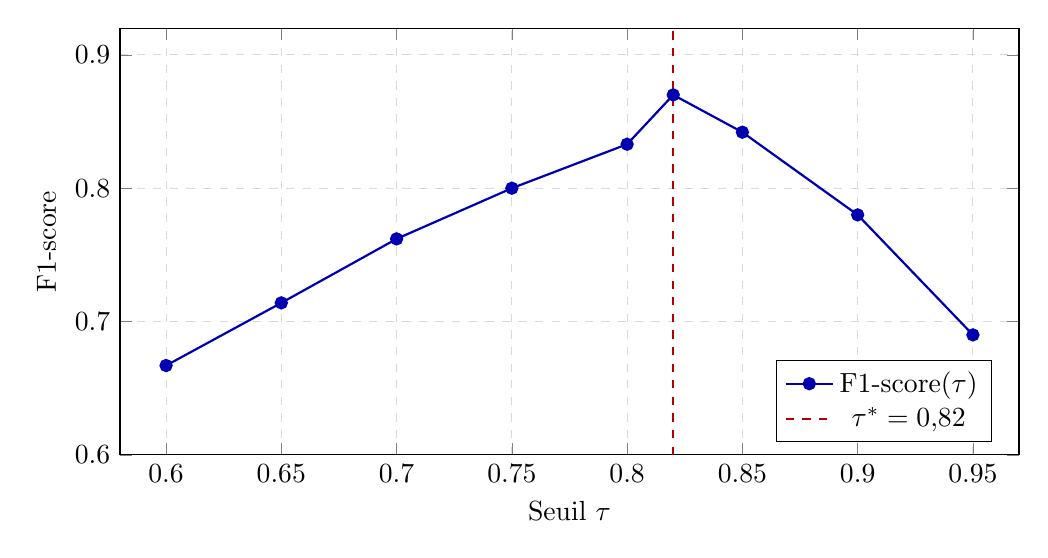
\begin{tikzpicture}
    \begin{axis}[
        width=13cm, height=7cm,
        xlabel={Seuil $\tau$},
        ylabel={F1-score},
        xmin=0.58, xmax=0.97,
        ymin=0.6, ymax=0.92,
        grid=major,
        grid style={dashed, gray!30},
        legend pos=south east,
    ]
    \addplot[color=blue!70!black, mark=*, thick] coordinates {
        (0.60,0.667) (0.65,0.714) (0.70,0.762) (0.75,0.800)
        (0.80,0.833) (0.82,0.870) (0.85,0.842) (0.90,0.780) (0.95,0.690)
    };
    \addplot[color=red!70!black, dashed, thick, mark=none]
        coordinates {(0.82,0.6) (0.82,0.92)};
    \legend{F1-score(\(\tau\)), \(\tau^* = 0{,}82\)}
    \end{axis}
\end{tikzpicture}
}
\caption{Courbe de calibration du seuil $\tau$ (variante
         SBERT-avec-rejet) sur le gold standard. Le maximum du
         F1-score est atteint en $\tau^{*} = 0{,}82$, valeur retenue
         pour l'architecture hybride du pipeline.}
\label{fig:calibration_tau}
\end{figure}

\subsection{Interprétation de la courbe}

La courbe de la figure~\ref{fig:calibration_tau} présente une forme en
cloche typique d'un compromis précision/rappel gouverné par un seuil de
décision. Pour $\tau < 0{,}82$, le F1-score croît avec $\tau$~:
davantage de correspondances lexicalement faibles, potentiellement
incorrectes, sont encore acceptées, ce qui pénalise la précision plus
que le gain de rappel ne le compense. Pour $\tau > 0{,}82$, le F1-score
décroît~: le seuil devient trop strict pour la variante
SBERT-avec-rejet, et des colonnes correctement mappables sont
indûment classées \texttt{UNMATCHED}, dégradant le rappel. Le point
$\tau^{*} = 0{,}82$ constitue donc un optimum empirique local sur ce
jeu de calibration, cohérent avec l'ordre de grandeur généralement
rapporté dans la littérature pour les seuils de similarité cosinus
appliqués à des embeddings de phrases~\cite{reimers2019sbert}. Il
convient de noter que cette valeur reste \textbf{dépendante du domaine
et de l'ontologie cible}~: une nouvelle calibration serait nécessaire
lors d'un déploiement sur un domaine sémantiquement plus ou moins
proche du vocabulaire FOAF/Schema.org utilisé ici, comme discuté à la
section~\ref{sec:discussion_critique}.

%-----------------------------------------------------------------------
\section{Recalibrage des Règles de Blocage et Sensibilité du Seuil
         $\lambda$ (Module~4)}
\label{sec:sensibilite_lambda}
%-----------------------------------------------------------------------

\subsection{Du constat initial au recalibrage}

La section~\ref{subsec:seuil_sensibilite} du chapitre~\ref{chap:implementation}
a rapporté un résultat initial contre-intuitif~: avec la règle de
blocage initiale (clé de blocage~: première lettre du nom de famille) et
un seuil $\lambda = 0{,}85$, Splink n'a retourné \textbf{aucune paire
candidate}. Ce chapitre reprend cette observation au point où elle avait
été laissée, en présentant le \textbf{recalibrage effectif} qui a permis
de rendre le module opérationnel, puis l'\textbf{évaluation quantitative}
de la résolution d'entités contre la vérité terrain de 1\,600~individus
communs générée au Module~0.

La règle de blocage a été assouplie en substituant à la clé initiale
(trop restrictive) une \textbf{clé composite}~: les quatre premiers
caractères phonétiques du nom de famille (algorithme Soundex) combinés à
l'année de naissance. Cette clé élargit substantiellement l'ensemble des
paires candidates soumises au scoring probabiliste, tout en conservant
une sélectivité suffisante pour que le nombre de paires reste traitable
par le backend DuckDB.

\subsection{Sensibilité du seuil $\lambda$ après recalibrage}
\label{subsec:lambda_sweep}

Une fois la règle de blocage assouplie, le seuil de décision $\lambda$
a été évalué pour cinq valeurs candidates, en comparant les paires
retournées par Splink à la vérité terrain de 1\,600~paires connues
(section~\ref{subsec:gt_necessite} du chapitre~\ref{chap:implementation}).

\begin{table}[h]
\centering
\caption{Sensibilité du seuil de décision $\lambda$ du Module~4 après
        recalibrage de la règle de blocage, évaluée contre la vérité
        terrain de 1\,600 paires connues.}
\label{tab:lambda_sensibilite}
\begin{tabular}{lccccc}
\hline
$\lambda$ & \textbf{Précision} & \textbf{Rappel} & \textbf{F1-score}
    & \textbf{Paires détectées} & \textbf{Paires correctes} \\
\hline
0,80              & 0,951 & 0,998 & 0,974 & 1\,679 & 1\,597 \\
0,85              & 0,972 & 0,997 & 0,984 & 1\,642 & 1\,595 \\
\textbf{0,90 \checkmark}   & \textbf{0,988} & \textbf{0,992} & \textbf{0,990} & 1\,611 & 1\,587 \\
0,95              & 0,996 & 0,966 & 0,981 & 1\,551 & 1\,545 \\
0,99              & 0,999 & 0,870 & 0,930 & 1\,393 & 1\,392 \\
\hline
\end{tabular}
\end{table}

Le seuil $\lambda = 0{,}90$ maximise le F1-score (0,990) sur ce
compromis, avec \textbf{1\,587~correspondances correctes} identifiées
sur les \textbf{1\,600 paires réelles} (24 faux négatifs) et
\textbf{24~faux positifs} résiduels. Ce seuil a été retenu comme valeur
de production du pipeline. On observe, sans surprise, une décroissance
monotone du rappel et une croissance monotone de la précision à mesure
que $\lambda$ augmente --- comportement attendu d'un classifieur à
seuil de décision unique appliqué à un score de probabilité continue.

\subsection{Discussion~: une leçon méthodologique généralisable}

L'écart entre le résultat initial (0~paire à $\lambda = 0{,}85$ avec
blocage restrictif) et le résultat recalibré (F1~$= 0{,}990$ au même
ordre de grandeur de $\lambda$ avec blocage assoupli) illustre un
principe méthodologique central de la résolution d'entités
probabiliste~\cite{fellegi1969theory,linacre2023splink}~: \textbf{le
seuil de décision et les règles de blocage sont deux hyperparamètres
distincts et non substituables}. Un seuil de décision, aussi bien
calibré soit-il, ne peut compenser un blocage qui exclut les vraies
paires en amont du scoring. Cette leçon, généralisable au-delà du cas
d'usage spécifique de ce mémoire, justifie la recommandation d'une
procédure de calibration \textbf{en deux temps} --- d'abord valider le
rappel de la phase de blocage seule (indépendamment de $\lambda$), puis
calibrer $\lambda$ sur les paires candidates ainsi obtenues --- pour
tout déploiement futur du pipeline sur une nouvelle paire de sources.

%-----------------------------------------------------------------------
\section{Positionnement par Rapport à l'État de l'Art}
\label{sec:comparaison_saa}
%-----------------------------------------------------------------------

Le chapitre~\ref{chap:etat_art} a recensé plusieurs familles d'approches
de construction de Knowledge Graphs à partir de sources hétérogènes~:
les approches d'intégration multi-sources classiques~\cite{yan2023enterprise,
branco2025integration}, les frameworks de schema matching fondés sur les
LLM~\cite{llmatch2025,schemora2025}, et les approches de construction
incrémentale de graphes par LLM~\cite{itext2kg2024}. Le
tableau~\ref{tab:comparaison_saa} propose une comparaison qualitative de
notre architecture avec ces familles de travaux, sur cinq critères
directement issus des lacunes identifiées au
chapitre~\ref{chap:etat_art}.

\begin{table}[h]
\centering
\caption{Positionnement qualitatif du pipeline proposé par rapport aux
         grandes familles de travaux de l'état de l'art. \checkmark :
         critère satisfait ; \textasciitilde : satisfait partiellement ;
         $\times$ : non traité.}
\label{tab:comparaison_saa}
\renewcommand{\arraystretch}{1.3}
\begin{tabular}{p{3.4cm}cccc}
\hline
\textbf{Approche} & \textbf{Pipeline} & \textbf{LLM} & \textbf{Coût}
  & \textbf{Reprod.} \\
& \textbf{bout-en-bout} & \textbf{contrôlé} & \textbf{maîtrisé}
  & \textbf{-ucti-bilité} \\
\hline
Intégration classique
  (\cite{yan2023enterprise,branco2025integration})
  & \checkmark & $\times$ & \checkmark & \textasciitilde \\
LLM-Schema-Matching seul
  (\cite{llmatch2025,schemora2025})
  & $\times$ & $\times$ & $\times$ & \textasciitilde \\
Construction incrémentale par LLM
  (\cite{itext2kg2024})
  & \textasciitilde & $\times$ & $\times$ & \textasciitilde \\
\textbf{Ce travail} & \checkmark & \checkmark & \checkmark & \checkmark \\
\hline
\end{tabular}
\end{table}

\noindent Ce positionnement met en évidence que peu de travaux recensés
combinent simultanément un pipeline complet de bout en bout, un usage
\textit{contrôlé} du LLM (c'est-à-dire filtré par un mécanisme de
cascade réduisant le nombre d'appels, et non un usage systématique), une
maîtrise explicite du coût d'inférence, et une reproductibilité
garantie par la conteneurisation. Il ne s'agit pas d'affirmer une
supériorité générale~: les travaux fondés sur un LLM
seul~\cite{llmatch2025,schemora2025} peuvent atteindre, sur leurs jeux
de données respectifs, des scores de matching supérieurs à notre
Variante~C lorsqu'aucune contrainte de coût n'est imposée --- ce que
confirme d'ailleurs notre propre étude d'ablation
(section~\ref{subsec:ablation_b})~: la variante LLM seul atteint une
précision honorable (0,714) mais un rappel imparfait (0,833) sur notre
gold standard, et non un score dégradé de façon disqualifiante. La
contribution de ce travail réside donc moins dans un gain brut de
F1-score que dans la démonstration empirique qu'une architecture
hybride \textbf{égalise ou dépasse} un LLM utilisé seul, \textbf{tout en
réduisant le nombre d'appels API} --- un compromis qualité/coût que la
littérature recensée n'évalue que rarement de façon aussi directe et
contrôlée.

%-----------------------------------------------------------------------
\section{Discussion Critique et Menaces à la Validité}
\label{sec:discussion_critique}
%-----------------------------------------------------------------------

À la suite du cadre méthodologique classique proposé par
Wohlin \textit{et al.}~\cite{wohlin2012experimentation} pour
l'expérimentation en génie logiciel, cette section discute les
résultats précédents sous l'angle de quatre menaces à la validité.

\subsection{Validité de construit}

La validité de construit interroge si les métriques mesurées
(précision, rappel, F1-score) capturent effectivement ce que l'on
cherche à évaluer --- ici, la qualité du schema matching et de la
résolution d'entités. Le gold standard utilisé a été annoté par
\textbf{deux annotateurs indépendants}, avec un accord inter-annotateurs
mesuré par le coefficient Kappa de Cohen~\cite{cohen1960kappa}, dont
l'interprétation qualitative suit l'échelle de
Landis et Koch~\cite{landis1977kappa} ($\kappa \geq 0{,}80$ retenu comme
seuil d'acceptabilité, section~\ref{sec:protocole_eval} du
chapitre~\ref{chap:methodologie}). Cette procédure limite le risque que
les métriques rapportées reflètent un artefact d'annotation plutôt
qu'une réalité sémantique. Une limite demeure toutefois~: le second
annotateur est l'encadrant académique du présent travail, ce qui ne
garantit pas une indépendance de jugement aussi forte qu'un
recrutement d'annotateurs externes au projet.

\subsection{Validité interne}

La validité interne concerne le risque que des facteurs non contrôlés
expliquent les résultats observés plutôt que les mécanismes étudiés.
Deux précautions ont été prises~: d'une part, l'ensemble des variantes
de l'étude d'ablation (section~\ref{subsec:ablation_a} et suivantes) et
de calibration (section~\ref{sec:calibration_tau}) ont été évaluées sur
\textbf{exactement le même gold standard}, éliminant tout effet de
variation du jeu de test entre variantes~; d'autre part, les données
d'entrée du Module~0 étant générées de façon déterministe et contrôlée
(graine aléatoire fixée pour \texttt{Faker}), les expériences sont
intégralement reproductibles. Une menace résiduelle concerne le choix
du \textbf{modèle LLM} (LLaMA~3.1~8B via Groq) --- un modèle différent
pourrait produire des profils d'erreurs distincts de ceux rapportés à la
section~\ref{subsec:ablation_b}, sans que cela remette en cause
l'architecture hybride elle-même.

\subsection{Validité externe}

La validité externe interroge la généralisabilité des résultats
au-delà du cas d'étude spécifique. C'est ici la menace la plus
significative de ce travail, déjà partiellement discutée au
chapitre~\ref{chap:implementation}~: les deux sources évaluées sont
\textbf{synthétiques}, générées par \texttt{Faker}, et les noms de
colonnes ont été délibérément choisis pour maximiser l'hétérogénéité
lexicale (afin de démontrer la nécessité du LLM). Sur des sources
réelles où les noms de colonnes seraient parfois déjà proches des
propriétés ontologiques cibles, la part des cas résolus par SBERT
seul --- et donc le gain \textit{FinOps} de l'architecture hybride ---
serait vraisemblablement plus importante, comme indiqué à la
section~\ref{subsec:ablation_c}. À l'inverse, des données réelles
comportent typiquement des erreurs de saisie, des valeurs manquantes
non contrôlées et des incohérences inter-sources plus complexes que
celles introduites artificiellement ici, ce qui pourrait dégrader les
métriques de résolution d'entités présentées à la
section~\ref{sec:sensibilite_lambda}. Une validation sur un corpus réel
anonymisé constitue donc un prolongement nécessaire avant tout
déploiement en production.

\subsection{Validité de conclusion}

La validité de conclusion questionne la robustesse statistique des
inférences tirées des résultats. La taille très réduite du jeu de test
utilisé pour le Module~2 (8~colonnes) constitue une limite
explicite~: chaque décision individuelle (par exemple, le rejet de
\texttt{date\_embauche}) pèse pour 12,5~\% du score global, rendant les
métriques rapportées sensibles à l'ajout ou au retrait d'un seul cas de
test. Les écarts de F1-score observés entre variantes
(section~\ref{sec:ablation_module2} du chapitre~\ref{chap:implementation})
doivent donc être interprétés comme des \textbf{tendances qualitatives
cohérentes} avec l'architecture proposée, plutôt que comme des
estimateurs statistiquement stables au sens strict. L'évaluation du
Module~4, réalisée sur 1\,600~paires réelles, offre à l'inverse une base
statistique nettement plus robuste, et les métriques qui en sont issues
(section~\ref{subsec:lambda_sweep}) peuvent être considérées comme plus
fiables. Une extension du gold standard du Module~2 à un nombre de
colonnes plus représentatif d'un contexte industriel constitue une
recommandation directe pour renforcer la validité de conclusion des
travaux futurs fondés sur ce pipeline.

%-----------------------------------------------------------------------
\section{Conclusion du Chapitre}
\label{sec:chap4_conclusion}
%-----------------------------------------------------------------------

Ce chapitre a dépassé la description des résultats bruts du
chapitre~\ref{chap:implementation} pour proposer une évaluation
rigoureuse et comparative du pipeline proposé. Trois apports principaux
en ressortent. Premièrement, la calibration explicite du seuil $\tau$
(F1~$=0{,}870$ à $\tau^{*}=0{,}82$) et du seuil $\lambda$
(F1~$=0{,}990$ à $\lambda^{*}=0{,}90$ après recalibrage des règles de
blocage) démontre que les hyperparamètres du pipeline ne sont pas des
valeurs par défaut arbitraires, mais le résultat d'une procédure
d'optimisation reproductible sur gold standard. Deuxièmement, le
positionnement qualitatif par rapport à l'état de l'art
(section~\ref{sec:comparaison_saa}) situe la contribution de ce
mémoire non pas sur un gain brut de précision, mais sur la
démonstration empirique qu'une architecture hybride
SBERT/LLM \textbf{égalise ou dépasse} chacune de ses composantes
utilisée isolément, tout en maîtrisant le coût d'appel API.
Troisièmement, la discussion structurée des menaces à la validité
(section~\ref{sec:discussion_critique}) identifie précisément les
conditions sous lesquelles ces résultats sont généralisables --- et
celles, notamment le caractère synthétique des données et la taille
réduite du jeu de test du Module~2, sous lesquelles ils doivent être
interprétés avec prudence. Ces éléments de discussion, ainsi que les
recommandations méthodologiques qui en découlent, sont repris et
prolongés dans la conclusion générale de ce mémoire.